%----------------------------------------------------------------------------------------
%	PACKAGES AND THEMES
%----------------------------------------------------------------------------------------
\documentclass[aspectratio=169,xcolor=dvipsnames]{beamer}
\usetheme{SimplePlus}
\setbeamertemplate{footline}[frame number]{}

\usepackage{hyperref}
\usepackage{graphicx} % Allows including images
\usepackage{booktabs} % Allows the use of \toprule, \midrule and \bottomrule in tables
\usepackage{siunitx}
\usepackage{import}
\usepackage{amsmath}
%\numberwithin{equation}{section}% numera eq come #section.#formula
\usepackage{amsthm}
\usepackage{stmaryrd}
\usepackage{amssymb}
\usepackage{wasysym}
\usepackage{cancel}
\usepackage{textcomp}
\usepackage{subcaption}
\definecolor{myred}{rgb}{0.545, 0.172, 0.031}
%\usepackage{cleveref}
%----------------------------------------------------------------------------------------
%	TITLE PAGE
%----------------------------------------------------------------------------------------

\title[short title]{Modelli computazionali multifisici} % The short title appears at the bottom of every slide, the full title is only on the title page
\subtitle{Poroelasticità e accoppiamenti chemo-meccanici}

\author[Pin-Yen] {Alessandro Mastrofini}

\institute[NTU] % Your institution as it will appear on the bottom of every slide, may be shorthand to save space
{
Meccanica Computazionale dei Tessuti e Biomateriali \\
Università degli Studi di Roma Tor Vergata% Your institution for the title page
}
\date{2022} % Date, can be changed to a custom date

\graphicspath{{figures/}} %Setting the graphicspat%h
\graphicspath{{figures/}} %Setting the graphicspath
\makeatletter
\providecommand*{\input@path}{}
\edef\input@path{{figures/}{}\input@path}% prepend
\makeatother
%----------------------------------------------------------------------------------------
%	PRESENTATION SLIDES
%----------------------------------------------------------------------------------------

\begin{document}

\begin{frame}
    % Print the title page as the first slide
    \titlepage
\end{frame}

%------------------------------------------------
\section{First Section}
%------------------------------------------------

\begin{frame}{Multiphysics}
\begin{figure}
\begin{minipage}{0.35\linewidth}
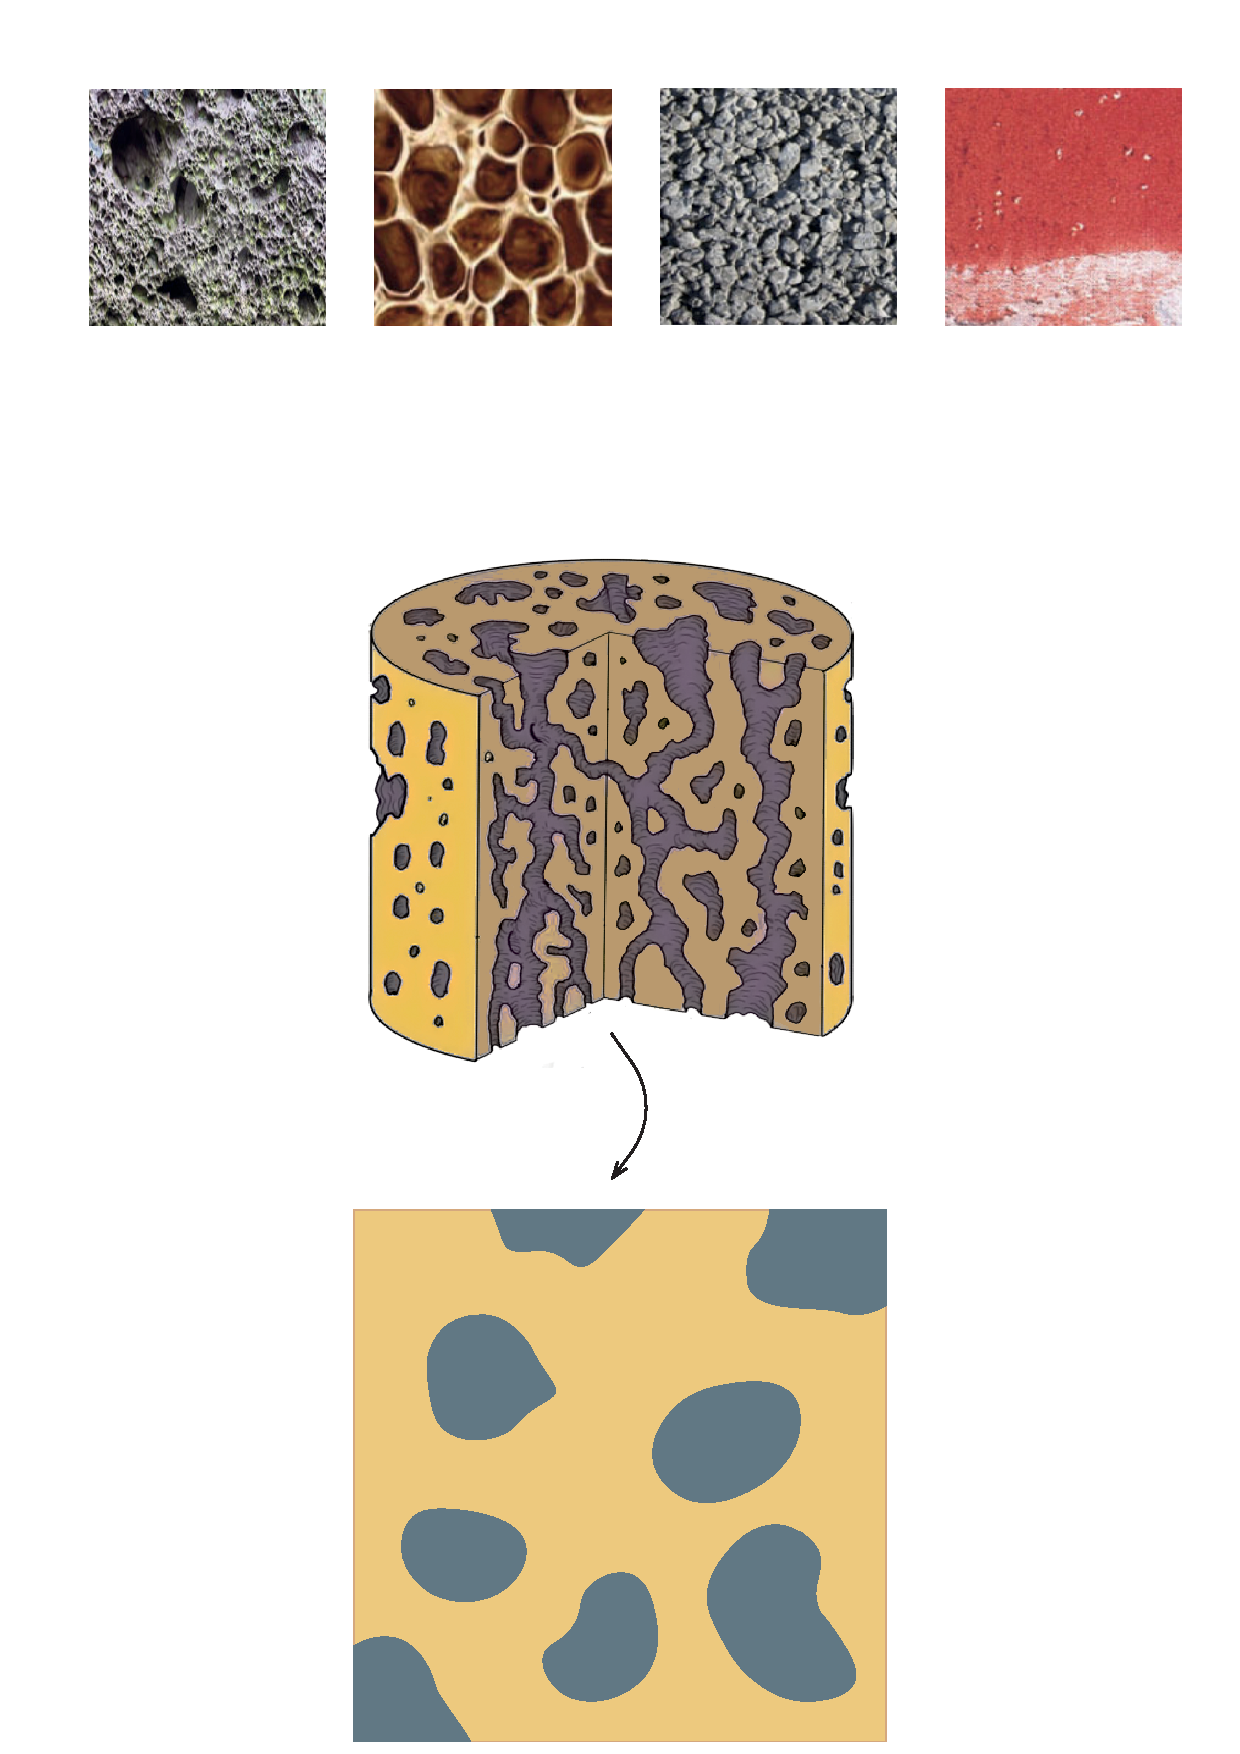
\includegraphics[width=\linewidth]{poroelasticity.pdf}
\end{minipage}\hfill
\begin{minipage}{0.65\linewidth}\centering
\begin{minipage}{0.4\linewidth}
	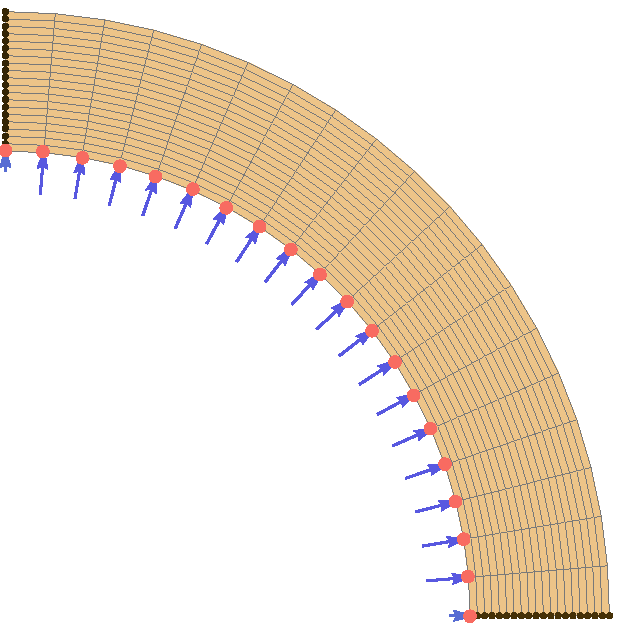
\includegraphics[width=\linewidth]{circularTest.pdf}
\end{minipage}\hspace{0.1\linewidth}
\begin{minipage}{0.45\linewidth}
	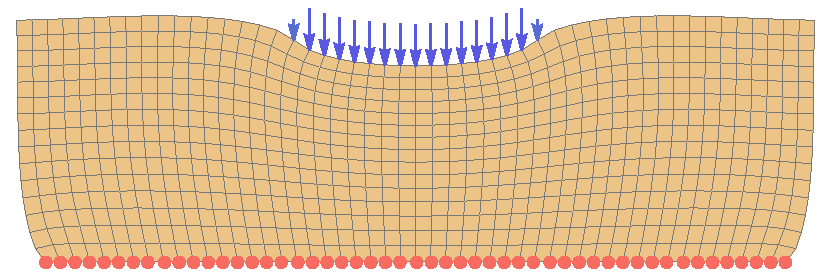
\includegraphics[width=\linewidth]{punchTest.pdf}
\end{minipage}
\end{minipage}
\end{figure}
\end{frame}

\begin{frame}{Uncoupled response}
\begin{figure}
	\begin{minipage}{\linewidth}
	\begin{minipage}{0.22\linewidth}\centering
	\tiny{\def\svgwidth{\linewidth}
	\input{circle_tex.pdf_tex}}
		\end{minipage}\hfill
	\begin{minipage}{0.3\linewidth}\centering
			\tiny{\def\svgwidth{\linewidth}
			\input{lambda_chemoelastic_tex.pdf_tex}}
\end{minipage}\hfill
		\begin{minipage}{0.3\linewidth}\centering
						\tiny{\def\svgwidth{\linewidth}
				\input{chemoelastic_deformed_tex.pdf_tex}}
	\end{minipage}
	\end{minipage}
\end{figure}
%%%%%%%%%
\begin{figure}
	\begin{minipage}{\linewidth}
		\begin{minipage}[b]{0.28\linewidth}\centering
						\tiny{\def\svgwidth{\linewidth}
				\input{displacement_chemo_tex.pdf_tex}}
		\end{minipage}\hfill
		\begin{minipage}[b]{0.32\linewidth}\centering
			\tiny{\def\svgwidth{\linewidth}
		\input{conc_1_tex.pdf_tex}}		
		\end{minipage}\hfill
		\begin{minipage}[b]{0.33\linewidth}\centering
			\tiny{\def\svgwidth{\linewidth}
		\input{conc_tex.pdf_tex}}		
		\end{minipage}
	\end{minipage}
\end{figure}
%%%%
\end{frame}

\begin{frame}{Poroelasticity}
	
	\begin{figure}
		\begin{minipage}{\linewidth}
			\begin{minipage}{0.3\linewidth}\centering
				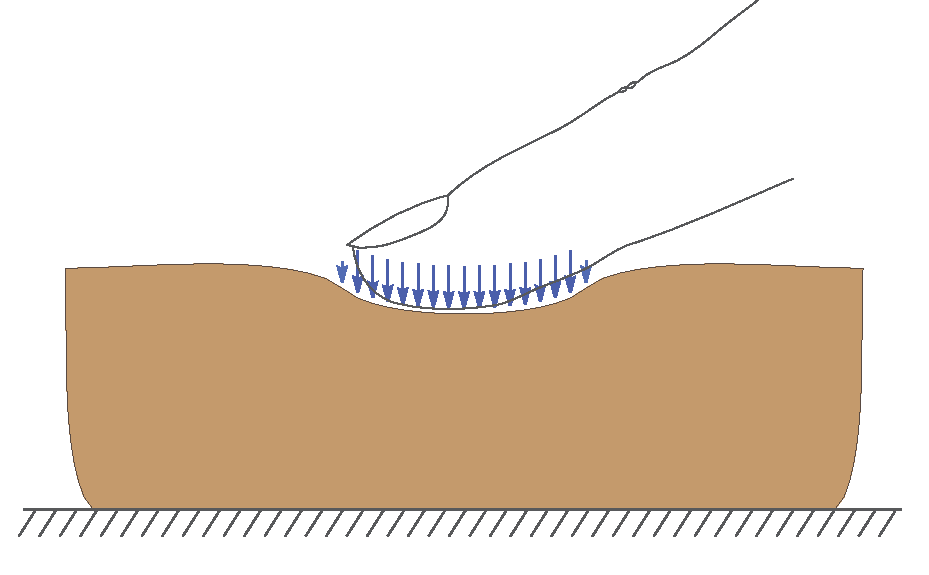
\includegraphics[width=\linewidth]{punch.pdf}
			\end{minipage}\hfill
			\begin{minipage}{0.3\linewidth}\centering

\tiny{$\Omega_{\mathrm{f}}\left(c-c_{0}\right)=\zeta=\alpha \varepsilon_{v o l}+\frac{p}{M}$}
\\\vspace{0.1\linewidth} 
\includegraphics[width=0.4\linewidth]{pores.pdf}
			\end{minipage}\hfill
			\begin{minipage}{0.3\linewidth}\centering
	 \fontsize{3pt}{4pt}\selectfont{\def\svgwidth{\linewidth}
	\input{lambda_poro.pdf_tex}}		
			\end{minipage}
		\end{minipage}
	\end{figure}

	\begin{figure}
	\begin{minipage}{\linewidth}
		\begin{minipage}{0.3\linewidth}\centering
			 \fontsize{3pt}{4pt}\selectfont{\def\svgwidth{\linewidth}
	\input{punch_frame_1_tex.pdf_tex}}		
		\end{minipage}\hfill
		\begin{minipage}{0.3\linewidth}\centering
	 \fontsize{3pt}{4pt}\selectfont{\def\svgwidth{\linewidth}
	\input{punch_frame_2_tex.pdf_tex}}		
		\end{minipage}\hfill
		\begin{minipage}{0.3\linewidth}\centering
	 \fontsize{3pt}{4pt}\selectfont{\def\svgwidth{\linewidth}
	\input{punch_frame_3_tex.pdf_tex}}		
		\end{minipage}
	\end{minipage}
\end{figure}

	\begin{figure}
	\begin{minipage}{\linewidth}		\hspace{0.01\linewidth}
		\begin{minipage}{0.6\linewidth}\centering
 \fontsize{3pt}{4pt}\selectfont{\def\svgwidth{\linewidth}
	\input{undrained_tex.pdf_tex}}	
		\end{minipage}\hfill
		\begin{minipage}{0.3\linewidth}\centering
	
 \fontsize{3pt}{4pt}\selectfont{\def\svgwidth{\linewidth}
	\input{undrained_v_tex.pdf_tex}}	
		\end{minipage}\hfill
	\end{minipage}
\end{figure}


\end{frame}

\begin{frame}{Drained conditions}

	\begin{figure}
	\begin{minipage}{\linewidth}
		\begin{minipage}{0.65\linewidth}\centering
			\begin{minipage}{\linewidth}
 \fontsize{3pt}{4pt}\selectfont{\def\svgwidth{0.9\linewidth}
	\input{total_displ_press_tex.pdf_tex}}	
			\end{minipage}\vspace{0.1\linewidth}
				\begin{minipage}{\linewidth}\hspace{0.01\linewidth}
			 \fontsize{3pt}{4pt}\selectfont{\def\svgwidth{\linewidth}
				\input{min_displ_press_tex.pdf_tex}}	
			\end{minipage}
		\end{minipage}\hfill
		\begin{minipage}{0.35\linewidth}\centering
\begin{minipage}{\linewidth}
				 \fontsize{3pt}{4pt}\selectfont{\def\svgwidth{\linewidth}
				\input{p_down_neg_tex.pdf_tex}}
\end{minipage}\\
\vspace{0.1\linewidth}
\begin{minipage}{\linewidth}
			 \fontsize{3pt}{4pt}\selectfont{\def\svgwidth{\linewidth}
		\input{p_down_null_tex.pdf_tex}} 
\end{minipage}\\
		\vspace{0.1\linewidth}			
	\begin{minipage}{\linewidth}
		 \fontsize{3pt}{4pt}\selectfont{\def\svgwidth{\linewidth}
	\input{p_down_pos_tex.pdf_tex}}	
	\end{minipage}\\
\vspace{0.05\linewidth}
\begin{flushleft}
 \fontsize{3pt}{4pt}\selectfont{\texttt{
SMTAddEssentialBoundary[\\  \quad Line[\{\{0,0\},\{L,0\}\},\textcolor{gray}{"p"}],1->Line[\{\textcolor{myred}{press}\}]] 
} }
\end{flushleft}
		\end{minipage}\hfill
	\end{minipage}
\end{figure}


\end{frame}


\begin{frame}{Asimmetry}
\begin{figure}
	\centering
	\scriptsize{right side}
		\begin{minipage}{\linewidth}
			\begin{minipage}{0.7\linewidth}\centering
	 \fontsize{3pt}{4pt}\selectfont{\def\svgwidth{0.95\linewidth}
	\input{right_pressure_tex.pdf_tex}}	
			\end{minipage}\hfill
			\begin{minipage}{0.3\linewidth}\centering
 \fontsize{3pt}{4pt}\selectfont{\def\svgwidth{\linewidth}
	\input{p_right_neg_tex.pdf_tex}}\vspace{0.03\linewidth}
 \fontsize{3pt}{4pt}\selectfont{\def\svgwidth{\linewidth}
	\input{p_right_pos_tex.pdf_tex}}	
			\end{minipage}\hfill
		\end{minipage}
	\centering
	\\\vspace{0.02\linewidth}
	\scriptsize{both side}
				\vspace{0.01\linewidth}\\
	\begin{minipage}{\linewidth}
		\begin{minipage}{0.5\linewidth}\centering
				\tiny{same BC}\\\vspace{0.03\linewidth}
				\begin{minipage}{0.45\linewidth}
					 \fontsize{3pt}{4pt}\selectfont{\def\svgwidth{\linewidth}
					\input{side_1_tex.pdf_tex}}
				\end{minipage}	\hspace{0.02\linewidth}
				\begin{minipage}{0.45\linewidth}
					 \fontsize{3pt}{4pt}\selectfont{\def\svgwidth{\linewidth}
					\input{side_2_tex.pdf_tex}}	
				\end{minipage}
			\vspace{0.03\linewidth}
			\\ \tiny{$\Delta p =1.5 ,\:\Delta v = 0.7$}
		\end{minipage}\hfill
		\begin{minipage}{0.5\linewidth}\centering
				\tiny{opposite BC}\\\vspace{0.03\linewidth}
				\begin{minipage}{0.45\linewidth}
				\fontsize{3pt}{4pt}\selectfont{\def\svgwidth{\linewidth}
					\input{opposite_1_tex.pdf_tex}}
			\end{minipage}	\hspace{0.02\linewidth}
			\begin{minipage}{0.45\linewidth}
				\fontsize{3pt}{4pt}\selectfont{\def\svgwidth{\linewidth}
					\input{opposite_2_tex.pdf_tex}}	
			\end{minipage}
			\vspace{0.03\linewidth}
						\\ \tiny{$\Delta p <10^{-15} ,\:\Delta v <10^{-15}$}
		\end{minipage}\hfill
	\end{minipage}
			\vspace{0.02\linewidth}\\
		\begin{minipage}{\linewidth}
				\begin{minipage}[c]{0.3\linewidth}\centering
\scriptsize{uncoupled response}\\\vspace{0.05\linewidth}  \fontsize{3pt}{4pt}\selectfont{\texttt{SMTAddEssentialBoundary[\textcolor{gray}{"p"}, 1 -> \textcolor{myred}{0}]];}}
			\end{minipage}\hfill
	\begin{minipage}[c]{0.3\linewidth}\centering
	\fontsize{3pt}{4pt}\selectfont{\def\svgwidth{\linewidth}
	\input{p_null_tex.pdf_tex}}	
	\end{minipage}\hfill
	\begin{minipage}[c]{0.32\linewidth}\centering
	\fontsize{3pt}{4pt}\selectfont{\def\svgwidth{\linewidth}
	\input{p_null_displ_tex.pdf_tex}}	
	\end{minipage}\hfill
\end{minipage}
\end{figure}
\end{frame}

\end{document}